\section{E/R diagram}
E/R diagram to represent the conceptual database design for the application.

\begin{figure}[H]
    \centering
    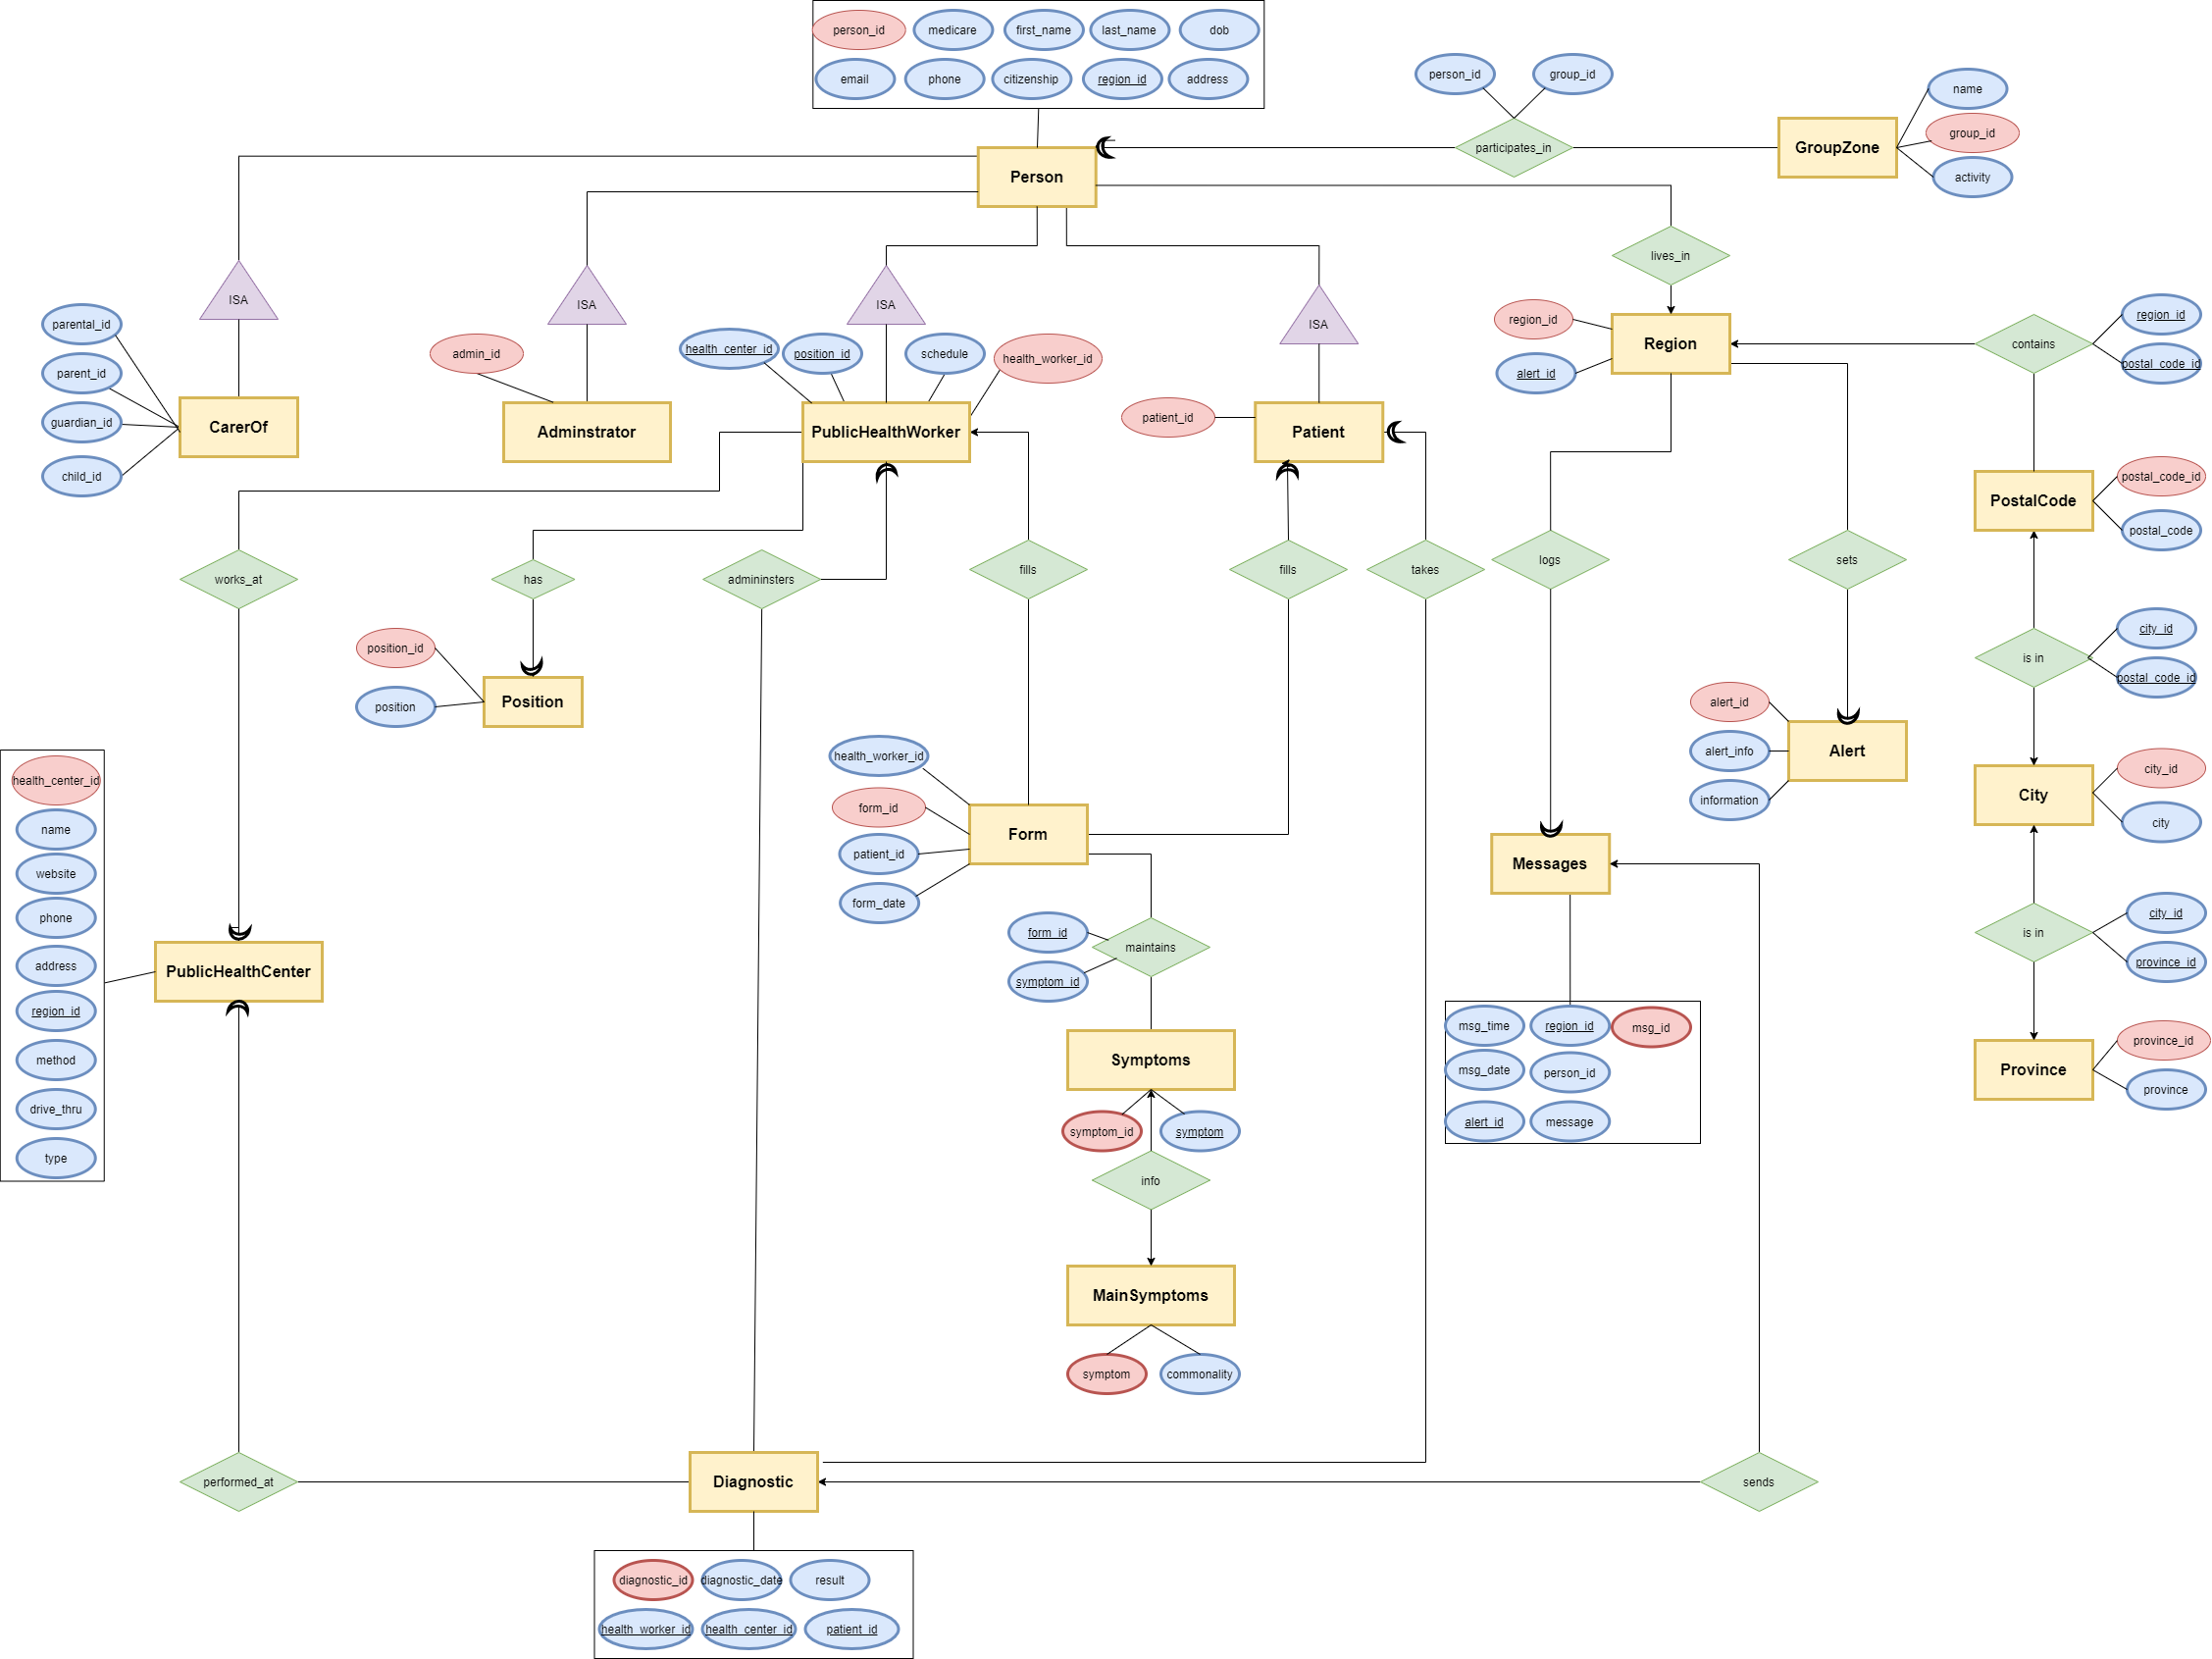
\includegraphics[scale=0.22]{imgs/ERD.PNG}
    \caption{E/R diagram}
\end{figure}

\subsection{Constraints captured by the diagram}
\begin{itemize}
    \item Multiplicity of relationships (pointed arrow)
    \item Inheritance (Triangle)
    \item Referential Integrity (Curved arrow)
    \item Primary keys (red bubble)
    \item Foreign keys (underlined attribute)
\end{itemize}
\subsection{Constraints not captured by the diagram}
One of the limitations we came across when using this notation is having referential integrity and multiplicity pointing to the same entity and we had cases where referential integrity and multiplicity of relationships conflicted.
\begin{itemize}
    \item We prioritized showing the referential integrity constraint. 
    \item We did not show referential integrity on the ERD when it comes to inherited entity sets.
    \item The diagram does not capture data types.
    \item The diagram does not capture Nullable attributes.
    \item The diagram does not show functional dependencies.
\end{itemize} 
\subsection{A different notation}
\begin{figure}[H]
    \centering
    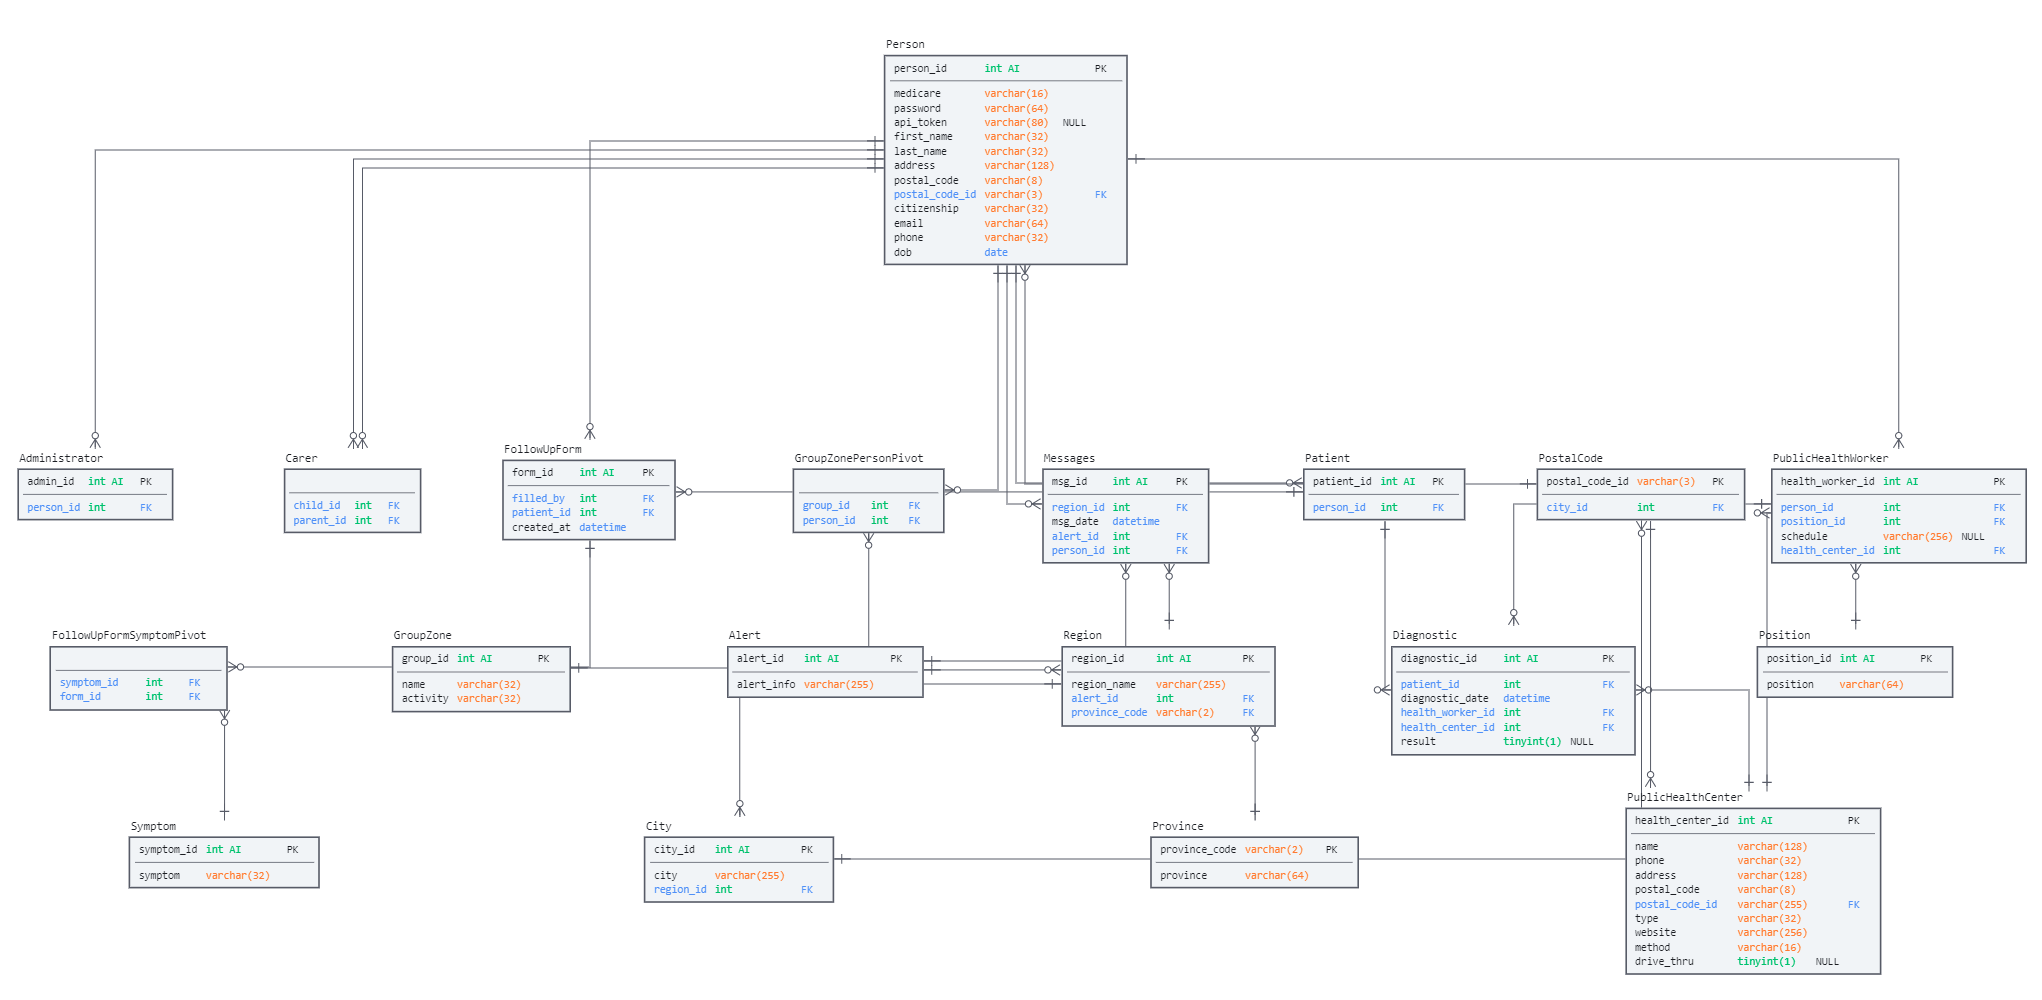
\includegraphics[scale=0.34]{imgs/nOtAnErD.png}
    \caption{A diagram that captures some more constraints (NOT AN ERD)}
\end{figure}